% !TEX program = lualatex

\documentclass[final]{beamer}

\usepackage[T1]{fontenc}
\usepackage{lmodern}
\usepackage[orientation=landscape,size=a0,scale=1.0]{beamerposter}
\usetheme{gemini}
\usecolortheme{oxford}
\usepackage{graphicx}
\usepackage{booktabs}
\usepackage{tikz}
\usepackage{pgfplots}
\usepackage[dvipsnames]{xcolor}
\pgfplotsset{compat=1.14}

% ====================
% Lengths
% ====================

% If you have N columns, choose \sepwidth and \colwidth such that
% (N+1)*\sepwidth + N*\colwidth = \paperwidth
\newlength{\sepwidth}
\newlength{\colwidth}
\setlength{\sepwidth}{0.025\paperwidth}
\setlength{\colwidth}{0.3\paperwidth}

\newcommand{\separatorcolumn}{\begin{column}{\sepwidth}\end{column}}

% ====================
% Title
% ====================

\title{Inverse-Free Sparse Variational Gaussian Processes}

\author{Stefano Cortinovis \inst{1} \and Laurence Aitchison \inst{2} \and Stefanos Eleftheriadis \inst{\ast, 3} \and Mark van der Wilk \inst{\ast, 1}}

\institute[shortinst]{\inst{1} University of Oxford \samelineand \inst{2} University of Bristol \samelineand \inst{3} No affiliation \and \inst{\ast} Equal contribution}

% ====================
% Footer (optional)
% ====================

\footercontent{
  \rlap{\href{mailto:cortinovis@stats.ox.ac.uk}{cortinovis@stats.ox.ac.uk}}\phantom{github.com/stefanocortinovis/relaxedgp} \hfill
  AISTATS 2026, Tangier, Morocco \hfill
  \href{https://github.com/stefanocortinovis/relaxedgp/}{github.com/stefanocortinovis/relaxedgp}}

% ====================
% Logo (optional)
% ====================

\logoright{
\includegraphics[height=10cm]{ox_logo.pdf}}
\logoleft{
\includegraphics[height=10cm]{qrcode_relaxedgp.pdf}}

% ====================
% Body
% ====================

\begin{document}

\begin{frame}[t]
\begin{columns}[t]
\separatorcolumn

% ============================================================
% COLUMN 1 — Setup & background
% ============================================================
\begin{column}{\colwidth}
    \begin{block}{Motivation}
        Gaussian processes (GPs) are flexible and convenient functional priors, but they suffer from \alert{computational limitations}.

        Even state-of-the-art sparse variational methods rely on
        {\Huge
            $$
                \mathbf{K}_{\mathbf{u}\mathbf{u}}^{\textcolor{red}{-1}}
            $$
        }
        
        \vspace{0.01cm}
        computed via Cholesky decompositions, which are:
        \begin{itemize}
            \setlength\itemsep{0.2cm}
            \item Ill-suited to \alert{low precision} arithmetic
            \item Inherently \alert{sequential}, unlike parallel \textit{matmuls}
            \item Computationally \alert{expensive} ($\mathcal{O}(M^3)$)
        \end{itemize}

        \begin{center}
            \LARGE\textbf{Can we train sparse variational GPs using \\ \alert{only matmuls}?}
        \end{center}
    \end{block}

    \begin{block}{Sparse variational Gaussian processes (SVGPs) \cite{hensman2013gaussian}}
        Apply variational inference to $f \sim \mathcal{GP}(0, k)$, $\mathbf{y} | \mathbf{f} \sim \prod_{n=1}^N p(y_n|f(\mathbf{x}_n))$:
        \begin{enumerate}
            \setlength\itemsep{0.4cm}
            \item Introduce $M \ll N$ \alert{inducing inputs} $\mathbf{Z}$ with outputs $\mathbf{u} = f(\mathbf{Z})$
            \item Define tractable variational \alert{posterior} (\textbf{M-SVGP})
            $$
                q(\mathbf{u}) = \mathcal{N}(\mathbf{m}, \mathbf{S}), \quad q(f(\cdot)) = \int p(f_{\neq{\mathbf{u}}}(\cdot) | \mathbf{u}) q(\mathbf{u})\ \mathrm{d}\mathbf{u}
            $$
            \item Formulate variational \alert{lower bound} (ELBO)
            \begin{equation*}
                \mathcal{L} = \sum_{n=1}^N \mathbb{E}_{\mathcal{N}(f_n; \textcolor{red}{\mu_n}, \textcolor{red}{\sigma_n^2})} \left[\log p(y_n | f_n)\right] - \textcolor{red}{\mathrm{KL}}\left[q(\mathbf{u}) \| p(\mathbf{u})\right]
            \end{equation*}
            \item \alert{Maximise} $\mathcal{L}(\mathbf{m}, \mathbf{S})$ to minimise $\mathrm{KL}[q(f)\|p(f|\mathbf{y})]$
        \end{enumerate}

        \begin{center}
            \Large \textbf{$\mathbf{K}_{\mathbf{u}\mathbf{u}}^{\textcolor{red}{-1}}$ shows up in $\textcolor{red}{\mu_n}$, $\textcolor{red}{\sigma_n^2}$, and in the $\textcolor{red}{\mathrm{KL}}$ term!}
        \end{center}

        \textbf{However}: we are free to reparameterise $\mathbf{m}$ and $\mathbf{S}$; e.g., the \textbf{L-SVGP} parameterisation \cite{panosFullyScalableGaussian2018} uses
        \begin{equation*}
            \mathbf{m} = \mathbf{K}_{\mathbf{u}\mathbf{u}} \tilde{\mathbf{m}}, \quad \mathbf{S} = (\mathbf{K}_{\mathbf{u}\mathbf{u}}^{-1} + \tilde{\mathbf{S}}^{-1})^{-1},
        \end{equation*}
        with $\tilde{\mathbf{S}}$ PD diagonal, inducing a bound $\hat{\mathcal{L}}(\tilde{\mathbf{m}}, \tilde{\mathbf{S}})$ with predictive variance $\textcolor{red}{\sigma_n^{2(\mathrm{L})}}$.
    \end{block}

    \begin{block}{Inverse-free variational bound (R-SVGP) \cite{vdwilk2022improved}}
        Let $\tilde{\mathbf{K}} := \mathbf{K}_{\mathbf{u}\mathbf{u}} + \tilde{\mathbf{S}}$ and introduce an auxiliary $\mathbf{T} \in \mathbb{R}^{M\times M}$. Reparameterise
        \begin{equation*}
            \mathbf{m} = \mathbf{K}_{\mathbf{u}\mathbf{u}} \tilde{\mathbf{m}}, \quad \mathbf{S} = \mathbf{K}_{\mathbf{u}\mathbf{u}} - \mathbf{K}_{\mathbf{u}\mathbf{u}}(2\mathbf{T} - \mathbf{T}\tilde{\mathbf{K}}\mathbf{T})\mathbf{K}_{\mathbf{u}\mathbf{u}},
        \end{equation*}
        giving
        \begin{equation*}
            \textcolor{ForestGreen}{\mu_n} = \mathbf{k}_{n\mathbf{u}}\tilde{\mathbf{m}}, \quad \textcolor{ForestGreen}{\sigma_n^2} = k_{nn} - \mathbf{k}_{n\mathbf{u}}(2\mathbf{T} - \mathbf{T}\tilde{\mathbf{K}}\mathbf{T})\mathbf{k}_{\mathbf{u}n},
        \end{equation*}
        and the closed-form KL upper bound
        \begin{equation*}
            \mathrm{KL}[q(\mathbf{u}) \| p(\mathbf{u})] \leq \tfrac{1}{2}\left(-\mathrm{tr}((2\mathbf{T} - \mathbf{T}\tilde{\mathbf{K}}\mathbf{T})\mathbf{K}_{\mathbf{u}\mathbf{u}}) - M + \tilde{\mathbf{m}}^\top \mathbf{K}_{\mathbf{u}\mathbf{u}} \tilde{\mathbf{m}} + \mathrm{tr}(\mathbf{T}\tilde{\mathbf{K}}) - \log|\mathbf{T}| - \log|\tilde{\mathbf{S}}|\right) =: \textcolor{ForestGreen}{\tilde{\mathrm{KL}}}
        \end{equation*}
        The resulting \emph{relaxed} bound $\tilde{\mathcal{L}}(\tilde{\mathbf{m}}, \tilde{\mathbf{S}}, \mathbf{T})$ is:
        \begin{itemize}
            \setlength\itemsep{0.3cm}
            \item A valid \alert{ELBO}
            \item \alert{Equivalent} to L-SVGP when $\mathbf{T} = \tilde{\mathbf{K}}^{-1}$
            \item \Large \underline{\alert{Free} of matrix \alert{inversion}/decomposition}
        \end{itemize}

        \textbf{Note}: using similar tricks, it is possible to derive (\emph{almost}) inverse-free bounds targeting other parameterisations, e.g., \textbf{W-SVGP} \cite{hensman2015mcmc}.
    \end{block}
\end{column}

\separatorcolumn

% ============================================================
% COLUMN 2 — Contributions
% ============================================================
\begin{column}{\colwidth}
\begin{alertblock}{Problem}
    \begin{center}
        \Large Joint optimisation of $\mathbf{T} = \mathbf{L}\mathbf{L}^\top$ with \alert{Adam} is terribly \alert{unstable}!
    \end{center}
\end{alertblock}

\begin{block}{Solution 1: Iterative matrix inversion via natural gradients}
    Tailored optimisation procedure for $\mathbf{T}$:
    \begin{itemize}
        \setlength\itemsep{0.6cm}
        \item Characterise $\mathbf{L}_{\tilde{\mathbf{K}}^{-1}} = \mathrm{chol}(\tilde{\mathbf{K}}^{-1})$ as the minimiser of an \alert{auxiliary loss}
        \begin{equation*}
            \mathbf{L}_{\tilde{\mathbf{K}}^{-1}} = \arg\min_{\mathbf{L}}\,\ell_{\tilde{\mathbf{K}}}(\mathbf{L}), \quad \ell_{\tilde{\mathbf{K}}}(\mathbf{L}) := \mathrm{KL}\!\left[\mathcal{N}(\mathbf{0}, \mathbf{L}\mathbf{L}^\top) \,\|\, \mathcal{N}(\mathbf{0}, \tilde{\mathbf{K}}^{-1})\right]
        \end{equation*}
        \item Compute the \alert{natural gradient} (NG) in closed form (\alert{matmuls only}):
        \begin{equation*}
            \tilde{\nabla}\ell_{\tilde{\mathbf{K}}} = \mathbf{L}\!\left[\mathrm{tril}(\mathbf{L}^\top \tilde{\mathbf{K}} \mathbf{L}) - \tfrac{1}{2}(\mathbf{I} + \mathrm{diag}(\mathbf{L}^\top \tilde{\mathbf{K}} \mathbf{L}))\right]
        \end{equation*}
        \item \alert{Alternate} $t^*$ NG steps on $\mathbf{L}$ with one Adam step on $\xi = \{\theta, \mathbf{Z}, \tilde{\mathbf{m}}, \tilde{\mathbf{S}}\}$
    \end{itemize}
    \textbf{Remark}: the NG update is an $\mathbf{L}$-space version of the classical Newton--Schulz iteration for $\tilde{\mathbf{K}}^{-1}$ $\rightarrow$ \alert{local quadratic convergence} by standard Newton-type arguments.
\end{block}

\begin{block}{Solution 2: Inducing-mean preconditioning}
    With NG updates for $\mathbf{T}$, R-SVGP $\approx$ L-SVGP $<$ W-SVGP:
    \begin{itemize}
        \setlength\itemsep{0.5cm}
        \item \textbf{Problem}: gap between L-SVGP and W-SVGP due to the \alert{inducing mean parameterisation}
        \begin{equation*}
            \mathbf{m} = \mathbf{K}_{\mathbf{u} \mathbf{u}} \tilde{\mathbf{m}}
        \end{equation*}
        \item \textbf{Solution for L-SVGP}: use $\mathbf{P}^{(\mathrm{L})} = \tilde{\mathbf{K}}^{-1}$ as a \alert{preconditioner} $\rightarrow$ i.e., use it to premultiply $\tilde{\mathbf{m}}$
        \item \textbf{Solution for R-SVGP}: use $\mathbf{P}^{(\mathrm{R})} = 2\mathbf{T} - \mathbf{T}\tilde{\mathbf{K}}\mathbf{T}$ as an \alert{inverse-free} preconditioner $\rightarrow$ $\mathbf{P}^{(\mathrm{R})}$ matches the L-SVGP gradients wrt $\xi$ when $\mathbf{T} = \mathrm{stopgrad}({\tilde{\mathbf{K}}^{-1}})$
    \end{itemize}
    \textbf{Note}: the naive choice $\mathbf{P}^{(\mathrm{R})} = \mathbf{T}$ would not work.
\end{block}

\begin{block}{Efficacy: toy datasets}
        Suffixes: \textbf{N} $=$ NG updates for $\mathbf{T}$; \textbf{P} $=$ inducing-mean preconditioning.
        \begin{figure}[h!]
            \centering
            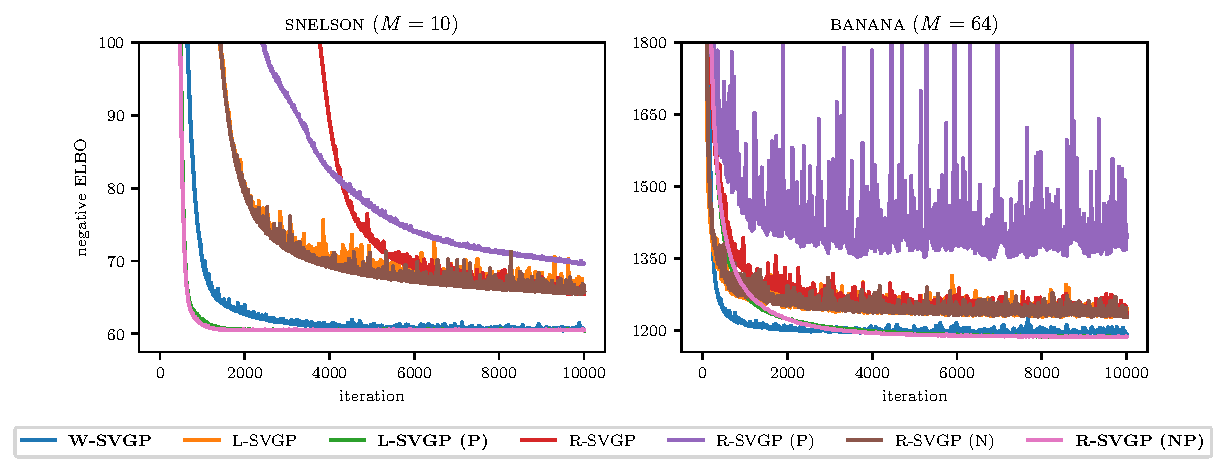
\includegraphics[width=1\textwidth]{figures/toy_trace.pdf}
            % Regenerate to match paper Fig. 1: 7 curves
            % (W-SVGP, L-SVGP, L-SVGP (P), R-SVGP, R-SVGP (P), R-SVGP (N), R-SVGP (NP))
        \end{figure}
        \textbf{R-SVGP (NP)} is the \alert{only} inverse-free variant that matches W-SVGP and L-SVGP (P).
    \end{block}

\begin{block}{Practical recipe for realistic datasets}
    \alert{Heuristics} that lower complexity of \textbf{bound evaluation} and keep the \textbf{NG inner loop} cheap:
    \begin{itemize}
        \setlength\itemsep{0.5cm}
        \item \textbf{Hutchinson}'s trace estimation with $K$ probes $\rightarrow$ bound evaluation in $\mathcal{O}((B + K)M^2)$
        \item \textbf{Regularise} $\mathbf{Z}$ updates: $k$-means++ initialisation, freeze during warmup, smaller LR, etc.
        \item \textbf{Stopping criteria} for $t^*$ with log-linear LR schedule
    \end{itemize}
    \centering Under these, $t^* \leq 3$ NG updates per step typically \alert{suffices} for shallow GPs on UCI datasets.
\end{block}
\end{column}

\separatorcolumn

% ============================================================
% COLUMN 3 — Results & discussion
% ============================================================
\begin{column}{\colwidth}
    \begin{block}{Efficiency: UCI runtime}
        NLPD vs wall-clock time on \textsc{elevators} ($N{=}16{,}599$) and \textsc{kin40k} ($N{=}40{,}000$). % Fixed NG step $\gamma = 1$; tolerance $\epsilon = 5\times 10^{-3}$; $K = 256$ Hutchinson probes.
        \begin{figure}[h!]
            \centering
            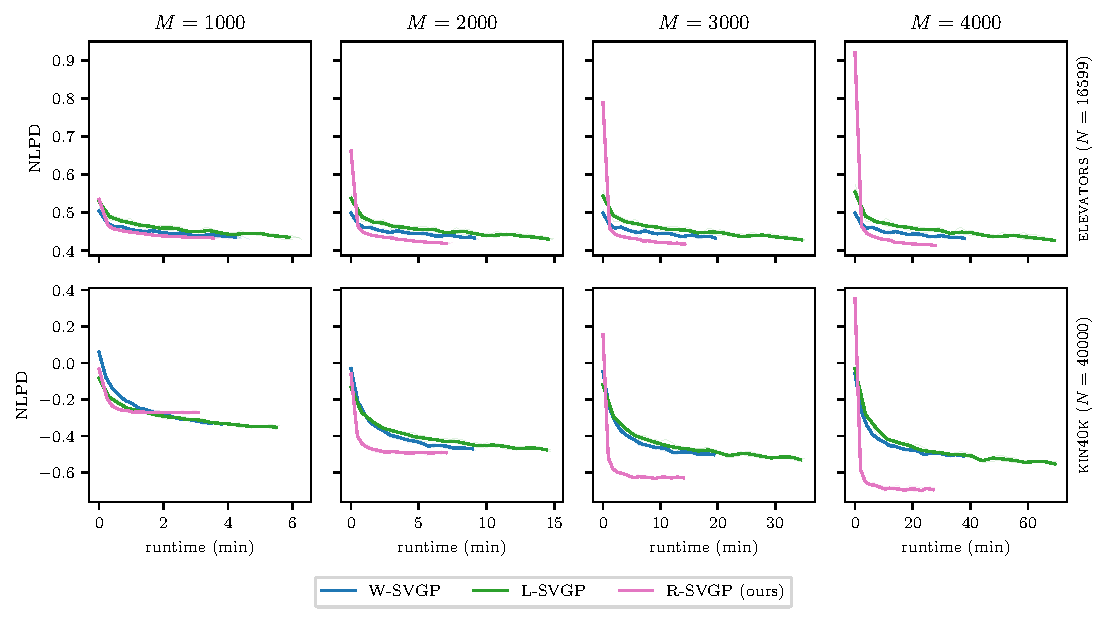
\includegraphics[width=0.98\textwidth]{figures/shallow_nlpd_seed.pdf}
            % Placeholder: paper Figure 2 (NLPD vs runtime, M ∈ {1000, 2000, 3000, 4000})
        \end{figure}
        \centering R-SVGP is up to \alert{$2.5\times$ faster than L-SVGP} and \alert{$1.4\times$ faster than W-SVGP}.
    \end{block}

    \begin{block}{Generality: deep GPs \& convolutional GPs}
        \small
        Test NLPD on \textsc{kin40k}, deep GPs with $L$ layers ($M = 500$):
        \begin{center}
        \begin{tabular}{cccc}
        \toprule
        $L$ & W-SVGP & L-SVGP & R-SVGP \\
        \midrule
        1 & $-0.38\,(0.001)$ & $-0.39\,(0.002)$ & $-0.39\,(0.002)$ \\
        2 & $-1.86\,(0.03)$  & $-1.88\,(0.02)$  & $-1.88\,(0.02)$  \\
        3 & $-2.39\,(0.03)$  & $-2.64\,(0.01)$  & $-2.64\,(0.01)$  \\
        \bottomrule
        \end{tabular}
        \end{center}

        Test error (\%) on \textsc{MNIST} ($M = 750$):
        \begin{center}
        \begin{tabular}{cccc}
        \toprule
        Kernel & W-SVGP & L-SVGP & R-SVGP \\
        \midrule
        RBF  & $1.96\,(0.02)$ & $1.95\,(0.01)$ & $1.94\,(0.02)$ \\
        Conv & $1.31\,(0.02)$ & $1.53\,(0.02)$ & $1.53\,(0.03)$ \\
        \bottomrule
        \end{tabular}
        \end{center}

        \centering \normalsize R-SVGP can be used as a \alert{drop-in replacement} within deep GPs and interdomain models.
    \end{block}

    \begin{block}{Discussion}
        First practical \alert{inverse-free} SVGP that trains stably on realistic datasets using \alert{only matmuls}, matches Cholesky-based baselines, and serves as a drop-in in deeper / interdomain models — with \alert{potential speed-ups} when well tuned.

        \textbf{Future directions:}
        \begin{itemize}
            \setlength\itemsep{0.15cm}
            \item \alert{Low-precision} (FP16/FP32) regimes where matmul advantages compound
            \item Inverse-free parameterisations targeting \alert{W-SVGP} directly
            \item Transfer of heuristics to deep / multi-output / interdomain settings
        \end{itemize}
    \end{block}

    \begin{block}{References}
        \footnotesize{\bibliographystyle{plain}\bibliography{references}}
    \end{block}

\end{column}

\separatorcolumn
\end{columns}
\end{frame}

\end{document}
